
	%Porque estudar este problema
\section{Conclusão}
%\begin{frame}{}
%	\centering \Huge \color{blue} \textbf{Justificativas}
%\end{frame}
	\begin{frame}{Tarefas Cumpridas}
		\begin{enumerate}
			\item \textbf{\textit{Driver}:}
			\begin{itemize}
				\item Concede a comunicação com o Arduino via USB por meio de funções de manipulação de arquivos situados no diretório {\tt /dev}.
			\end{itemize}
			\item \textbf{Arduino:} 
			\begin{itemize}
				\item Realiza seu papel de intermediário entre as extremidades:
				\begin{itemize}
					\item Tanto com o FPGA quanto com o \textit{Driver}.
				\end{itemize}
				\item Exibe as informações corretamente.
			\end{itemize}
			\item \textbf{FPGA:}
			\begin{itemize}
				\item É possível realizar a encriptação de \textbf{apenas 1 bloco de 64-bits por vez}:
				\begin{itemize}
					\item Sendo este alterado manualmente pelo usuário.
				\end{itemize} 
			\end{itemize}

			%\begin{itemize}
			%	\item \textit{Driver} \textit{Driver} dentro de um sistema operacional Linux;
			%	\item Comunicação através de protocolo USB;
			%\end{itemize} 
			%\item Desenvolver um \textit{Driver} simples e de fácil entendimento.
		\end{enumerate}
	\end{frame}
	\begin{frame}{Exemplo Prático}
		\begin{figure}[p]
			\centering
			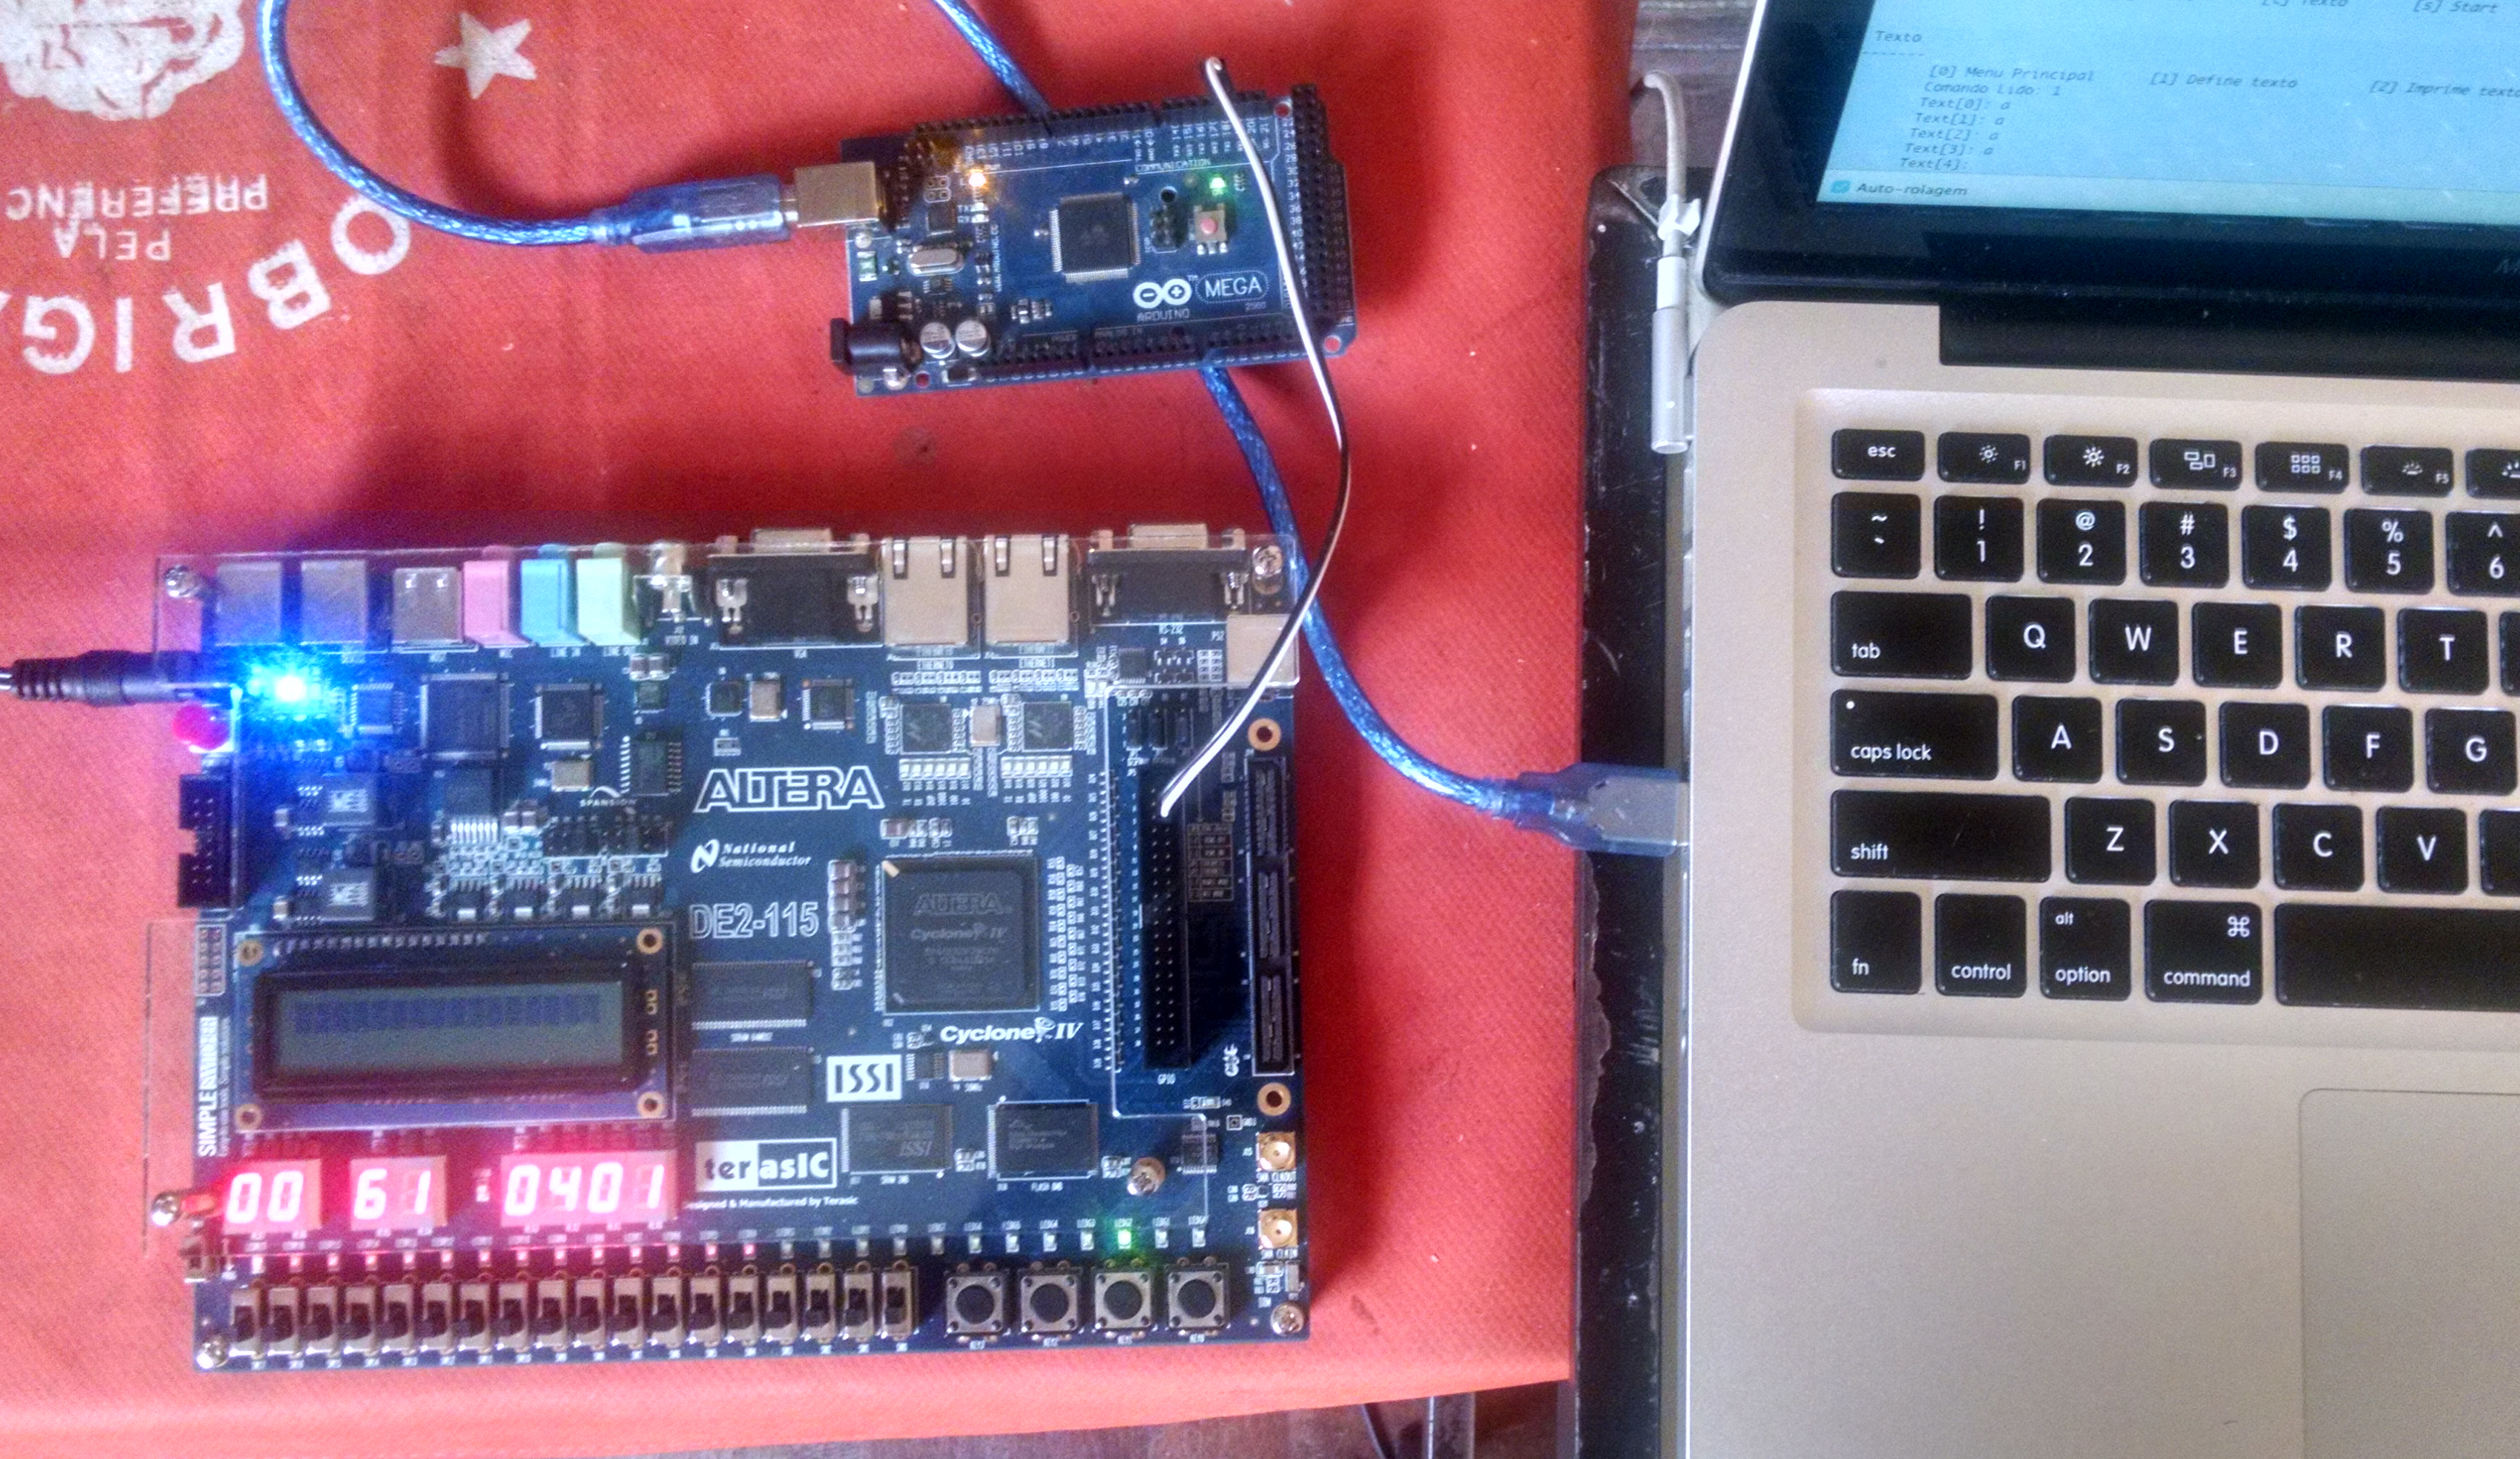
\includegraphics[width=1\textwidth]{img/projetoReal/real.jpg}
			\caption{Foto real do projeto em atuação.}
			\label{fig:projetoreal}
		\end{figure}
	\end{frame}
	\begin{frame}{Tarefas Pendentes}
		\begin{enumerate}
			\item Além da \textbf{encriptação}, adicionar o algoritmo que realiza a \textbf{decodificação}:
			\begin{itemize}
				\item Adicionar os procedimentos pra que a decriptação seja possível.
			\end{itemize}
			\item Atualmente encripta-se somente 1 bloco por vez (alterado manualmente pelo usuário):
			\begin{itemize}
				\item Permitir que o envie o texto do tamanho que quiser desde que:
				\begin{itemize}
					\item Seu limite seja a capacidade de armazenamento interno do Arduino.
				\end{itemize}
			\end{itemize}
			\item Desenvolver um conhecimento maior para aprimorar o \textit{Driver} TTY.

			%\begin{itemize}
			%	\item \textit{Driver} \textit{Driver} dentro de um sistema operacional Linux;
			%	\item Comunicação através de protocolo USB;
			%\end{itemize} 
			%\item Desenvolver um \textit{Driver} simples e de fácil entendimento.
		\end{enumerate}
	\end{frame}